%\section{対象計算領域の設定} \label{sec:domain}
\section{\SecBasicDomainSetting} \label{sec:domain}
%=======================================================================

本節では、格子数、計算領域とそのMPIプロセスとの関係を説明する。
計算領域は、水平格子間隔と格子点数およびMPIプロセス数によって決定される。
この関係を図\ref{fig:domain}に示す。
水平方向に2次元の領域分割を行うことで並列化がなされている。

格子点数およびMPIプロセス数は、
\namelist{PARAM_ATMOS_GRID_CARTESC_INDEX}内の\nmitem{IMAX, JMAX}、\\
\namelist{PARAM_PRC_CARTESC}内の\nmitem{PRC_NUM_X, PRC_NUM_Y}で設定する。
図\ref{fig:domain}に示すように、計算領域全体は、
\XDIR に\nmitem{PRC_NUM_X}個、\YDIR に\nmitem{PRC_NUM_Y}個に分割される。
プロセス数はゼロから始まり、左下から右上の順で番号付けされる(図\ref{fig:domain}における矢印)。
分割された各領域は1つのMPIプロセスによって担当され、各MPIプロセスは\nmitem{IMAX, JMAX, KMAX}個の格子ブロックを受け持つ。
ここで注意すべきことは、「指定する格子点数は各プロセスが受け持つ値」であり、計算領域全体の格子点数ではないことである。
別の言い方をすれば、計算領域全体は、水平格子間隔、格子点数、MPIプロセス数に依存する。

したがって、各方向の格子点と総格子点数は、以下のように計算される。
\begin{eqnarray}
&& {\rm 領域内{\XDIR} の格子数} = \verb|IMAX| \times \verb|PRC_NUM_X|
   \label{eq:xgridnum}\\
&& {\rm 領域内{\YDIR}の格子数} = \verb|JMAX| \times \verb|PRC_NUM_Y|
   \label{eq:ygridnum}\\
&& {\rm 領域内の総格子数} = \left(\verb|IMAX| \times \verb|PRC_NUM_X|\right)
   \times (\verb|JMAX| \times \verb|PRC_NUM_Y|)
   \times (\verb|KMAX| )  \nonumber
\end{eqnarray}
ここで、\nmitem{KMAX}は鉛直方向の格子点数であり、
\namelist{PARAM_ATMOS_GRID_CARTESC_INDEX}内で指定する。

また、領域全体の大きさは、式(\ref{eq:xgridnum}、\ref{eq:ygridnum})を使って、
\begin{eqnarray}
&& \rm{{\XDIR}の領域の長さ} = \rm{{\XDIR}の格子点数} \times \verb|DX| \nonumber\\
&& \rm{{\YDIR}の領域の長さ} = \rm{{\YDIR}の格子点数} \times \verb|DY| \nonumber
\end{eqnarray}
と決定される。ここで、第\ref{subsec:gridinterv}節で記述したように、
\nmitem{DX, DY}は\namelist{PRAM_ATMOS_GRID_CARTESC}内で指定する。
水平方向の解像度と領域の大きさを設定し、利用する MPI プロセス数を与えた場合は、
1 つのMPIプロセスが受け持つ格子点数は上記の関係から決められる。

次の小節では、MPIプロセス数、格子数、格子間隔の設定をより詳しく説明する。
\textcolor{blue}{これらの設定は\texttt{pp.conf}、\texttt{init.conf}、\texttt{run.conf}の設定ファイル間で一致させなければならない}
ことに注意が必要である。

\begin{figure}[h]
\begin{center}
  \includegraphics[width=0.8\hsize]{./figure/domain_decomposition_v2.png}\\
  \caption{計算領域全体に対する、水平格子間隔(\texttt{DX}, \texttt{DY})、MPIプロセスあたりの格子数(\texttt{IMAX}, \texttt{JMAX})、MPIプロセス数(\texttt{PRC\_NUM\_X}, \texttt{PRC\_NUM\_Y})の関係。水色の領域は、1つのMPIプロセスが担当する領域に対応する。}
  \label{fig:domain}
\end{center}
\end{figure}

%-----------------------------------------------------------------------
\subsection{\SubsecMPIProcess} \label{subsec:relation_dom_reso2}
%-----------------------------------------------------------------------

MPIプロセス数は設定ファイルの\namelist{PARAM_PRC_CARTESC}内で指定する。
\scalerm の入出力ファイルはMPIプロセス毎に分割されているため、
分割ファイルの総数はMPIプロセス数によって変化する。
例えば、2-MPI並列用に作成した初期値ファイルは、
4-MPI並列のモデル実行には使用できない。
MPIプロセス数を変更する場合は、
\verb|pp.conf|、\verb|init.conf|、\verb|run.conf| 内の
\namelist{PARAM_PRC_CARTESC}を編集し、
\verb|pp|、\verb|init| の過程を再度行う必要がある。
\editboxtwo{
\verb|&PARAM_PRC| & \\
\verb| PRC_NUM_X       = 2,| & ; {\XDIR}(東西方向)のMPI並列分割数 \\
\verb| PRC_NUM_Y       = 1,| & ; {\YDIR}(南北方向)のMPI並列分割数 \\
\verb|/|\\
}

MPI プロセスの総数は、\verb|PRC_NUM_X| $\times$ \verb|PRC_NUM_Y|  によって与えられる。
上記の例では、\XDIR に領域を2分割し、\YDIR には領域を分割しないので、
2-MPI 並列ということになる。
ジョブを投げる際のMPIコマンドに指定するMPIプロセス数として、この総プロセス数を与える必要がある。
この条件を満たさない場合には、プログラムは計算を行わずに直ちに終了し、
下記のメッセージが標準出力に出力される。
\msgbox{
\verb|xxx total number of node does not match that requested. Check!| \\
}

%-----------------------------------------------------------------------
\subsection{\SubsecGridNumSettng} \label{subsec:relation_dom_reso3}
%-----------------------------------------------------------------------

格子数は、設定ファイル(\verb|***.conf|)の\namelist{PARAM_ATMOS_GRID_CARTESC_INDEX}で指定する。
指定する水平格子数は、1つのMPIプロセス当たりの値であることに注意が必要である。
\editboxtwo{
\verb|&PARAM_ATMOS_GRID_CARTESC_INDEX| & \\
\verb| KMAX = 97,|  & ; 鉛直層数 \\
\verb| IMAX = 20,|  & ; プロセスあたりの{\XDIR}の格子点数 \\
\verb| JMAX = 25,|  & ; プロセスあたりの{\YDIR}の格子点数 \\
\verb|/|\\
}

%-----------------------------------------------------------------------
\subsection{\SubsecGridIntvSettng} \label{subsec:gridinterv}
%-----------------------------------------------------------------------

第\ref{subsec:buffer}節で述べる緩和領域を除いて水平格子間隔は等間隔でのみ設定できるが、
鉛直格子間隔は任意に設定できる。
全方向について格子間隔を等間隔で設定する場合には、
\namelist{PARAM_ATMOS_GRID_CARTESC}内の\nmitem{DX, DY, DZ}にそれぞれ、
東西、南北、鉛直方向の格子間隔を指定する(単位は[m])。
\editboxtwo{
\verb|&PARAM_ATMOS_GRID_CARTESC| & \\
\verb| DX = 500.D0,| & ; {\XDIR}(東西方向)の格子間隔\\
\verb| DY = 500.D0,| & ; {\YDIR}(南北方向)の格子間隔\\
\verb| DZ = 500.D0,| & ; {\ZDIR}(鉛直方向)の格子間隔\\
\verb|/|\\
}

以下の囲みに、等間隔でない格子系を指定する方法を示す。
モデルはローレンツ格子を採用しており、
速度ベクトルと他のスカラー量に対する定義点は半格子分ズレている。
ここでは、スカラー量の位置をセンターポイントと呼び、
それから半格子ズレた位置をフェイスポイントと呼ぶ。
鉛直格子点の位置を直接指定する場合は、
\namelist{PARAM_ATMOS_GRID_CARTESC}内の\nmitem{FZ(:)}に配列として与えればよい
\footnote{この場合には、シミュレーションで用いられたものと同じ浮動小数点の精度を用いることが望ましい。
デフォルトでは、モデルは倍精度の浮動小数点を使用するとしてコンパイルされる。
}。
詳細は図\ref{fig:scale_grid}を参照されたい。
また、\nmitem{FZ(:)}で指定する要素の数は、鉛直層数
(\namelist{PARAM_ATMOS_GRID_CARTESC_INDEX}内の\nmitem{KMAX})と一致している必要があることに注意が必要である。
例として、理想実験の設定ファイルを下記に示す。
\editboxtwo{
\verb|&PARAM_ATMOS_GRID_CARTESC|     & \\
\verb| DX = 500.D0,|   & {\XDIR} の格子間隔(等間隔) [m]\\
\verb| DY = 500.D0,|   & {\YDIR}の格子間隔(等間隔) [m]\\
\verb| FZ(:) = |       & {\ZDIR}のフェイスポイントの位置 [m] \\
\verb|    80.000000000000000      ,| & \\
\verb|    168.00000190734863      ,| & \\
\verb|    264.80000610351567      ,| & \\
\verb|     〜 中略 〜|           & \\
\verb|    14910.428862936289      ,| & \\
\verb|    15517.262523292475      ,| & \\
\verb|    16215.121232702089      ,| & \\
\verb|    17017.658748523147      ,| & \\
\verb|    17940.576891717363      ,| & \\
\verb|    19001.932756390710      ,| & \\
\verb|    20222.492000765058      ,| & \\
\verb| BUFFER_DZ = 5000.D0,|          & 第\ref{subsec:buffer}節参照\\
\verb| BUFFFACT  =   1.0D0,|          & 第\ref{subsec:buffer}節参照\\
\verb|/|\\
}

\begin{figure}[tb]
\begin{center}
  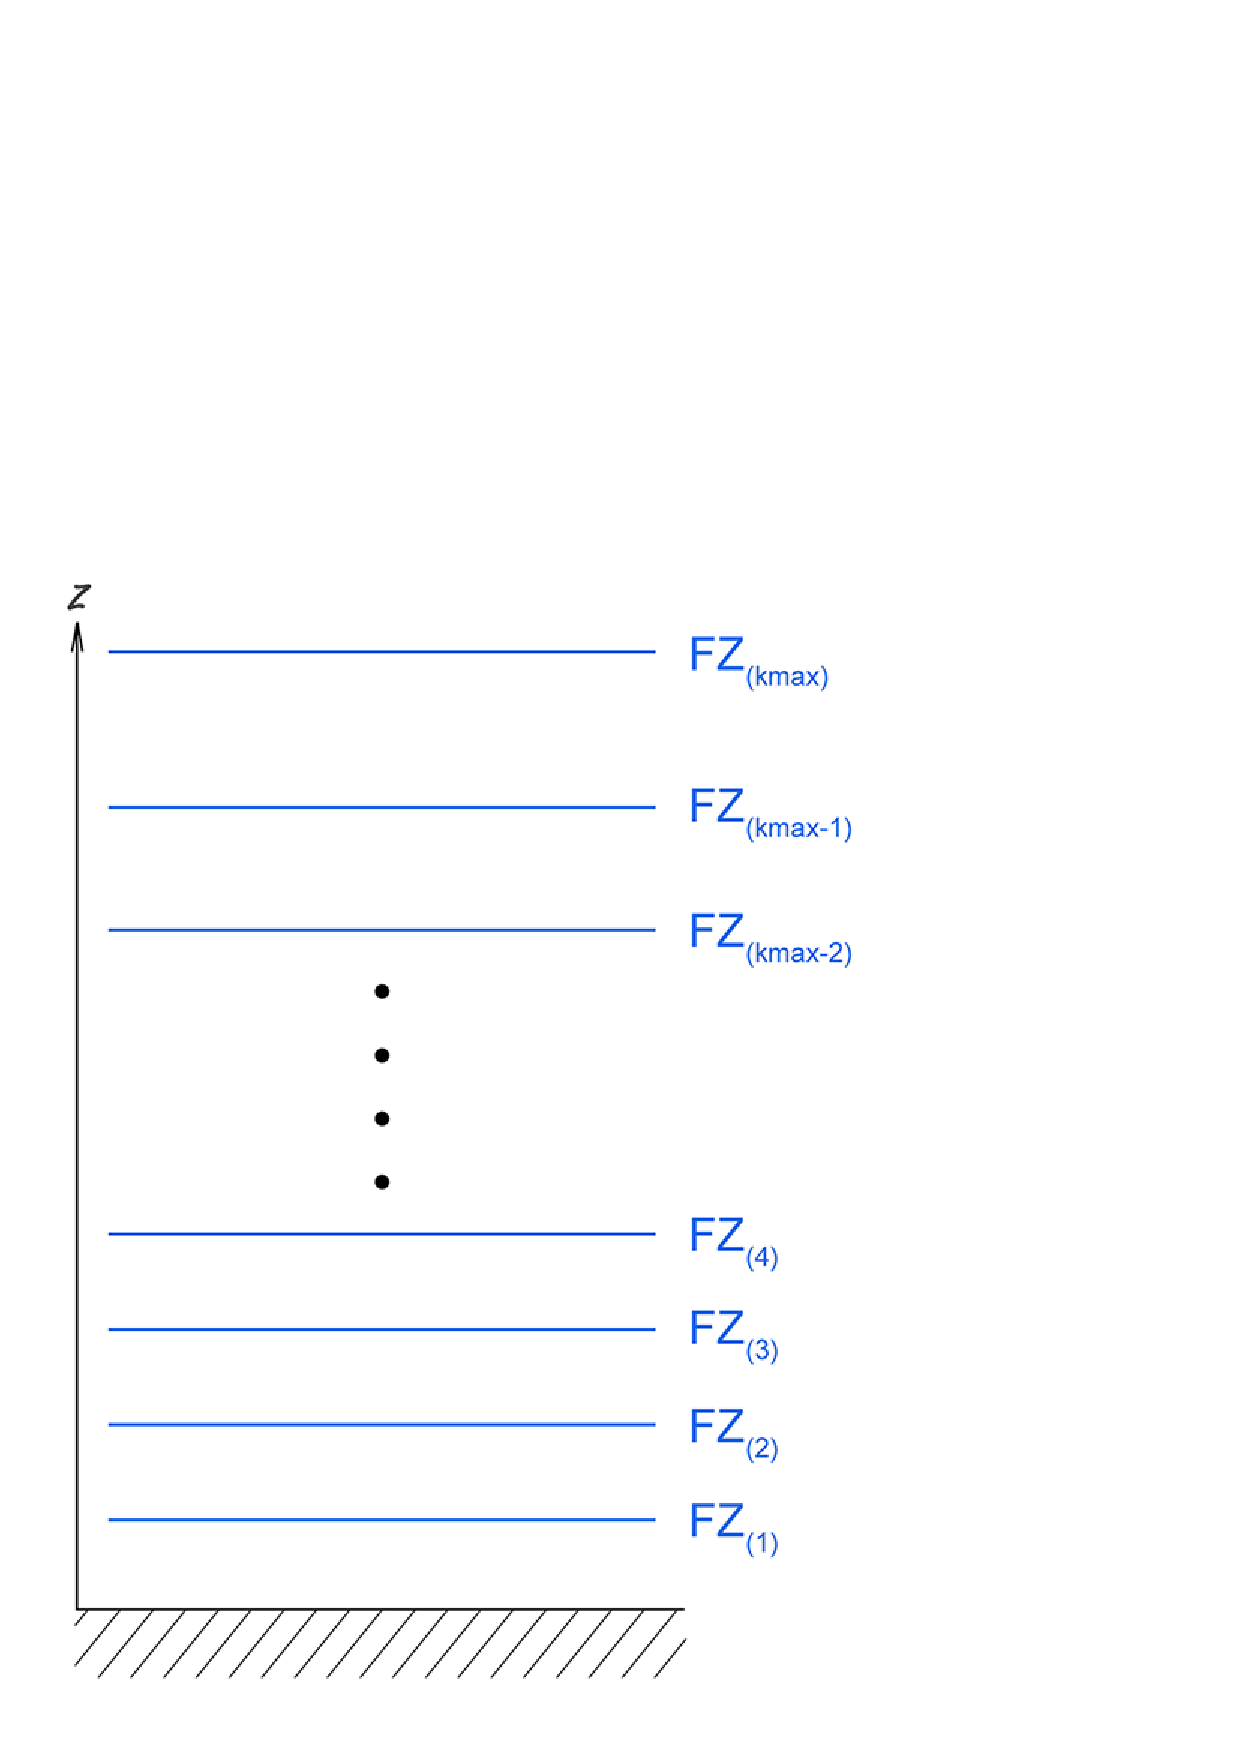
\includegraphics[width=0.4\hsize]{./figure/verticalface.pdf}\\
  \caption{\scalerm におけるフェイスポイントの定義点。
  \namelist{PARAM_ATMOS_GRID_CARTESC}で\nmitem{FZ}を指定する時は、
  $k=1$での値として第1層目上端の高さを与える。$k=1$での値は地表面の高さでないことに注意が必要である。}
  \label{fig:scale_grid}
\end{center}
\end{figure}

上記の設定は、標高 0 m の場所で処理される。
地形が存在する場所での鉛直格子点の位置は、地形に沿った座標系によって適切に取り扱われる。


鉛直格子点の位置は任意に設定できるが、変わった設定をすると計算不安定がしばしば生じる。
これを避けるために、ディレクトリtexttt{scale-\version/scale-rm/util/makevgrid/}の中に
\verb|make_vgrid.f90|というFortranプログラムと幾つかのネームリストの例を用意している。
必要があれば参考として用いることができる。
このツールは\nmitem{FZ(:)}の値を直接出力するので、コピーして設定ファイルに貼り付けると良いだろう。

%-----------------------------------------------------------------------
\subsection{\SubsecRayleighDampingSetting} \label{subsec:raydamp}
%-----------------------------------------------------------------------

\scalerm は高度座標を採用している。
最上層の境界条件は剛体壁であり、モデル上端において音波や重力波がしばしば反射する。
反射波の悪影響を軽減するために、モデル領域の上部に「スポンジ層」と呼ばれる減衰層を設ける。
スポンジ層内では、レイリー摩擦によって鉛直速度を減衰させる。
緩和の時定数(e-folding time)はモデル上端で最も短く、高度が下がるにつれて長くする。
スポンジ層の下端より下では、緩和の時定数は無限大に設定する。
スポンジ層の厚さの指定方法は2種類あり、\namelist{PARAM_ATMOS_DYN}で設定する。
\begin{enumerate}
\item スポンジ層の層数を指定\\
  \nmitem{ATMOS_DYN_wdamp_layer} でスポンジ層の層数を指定する。
  この層数はモデル上端から数える。
\item スポンジ層の下端高度[m]の指定\\
  \nmitem{ATMOS_DYN_wdamp_height} で指定した高度よりも上部にある層を、スポンジ層として設定する。
\end{enumerate}

デフォルトでは上記のパラメータは両方とも設定されず、スポンジ層は適用されない、
両方が指定された場合は、\nmitem{ATMOS_DYN_wdamp_layer} が優先される。

スポンジ層上端での緩和の時定数は、\nmitem{ATMOS_DYN_wdamp_tau} で設定する(単位は秒)。\\
これには\nmitem{TIME_DT_ATMOS_DYN}よりも小さな値は設定できない。
時定数を陽に指定しない場合は、\nmitem{TIME_DT_ATMOS_DYN} の10倍の値が自動で設定される。
\nmitem{TIME_DT_ATMOS_DYN}については、第\ref{sec:timeintiv}節を参照されたい。
また、具体的な設定例は、第\ref{subsec:atmos_dyn_scheme}節を参照されたい。

%鉛直格子を一定間隔に設定する(第\ref{subsec:gridinterv}節参照)場合にも、スポンジ層の格子間隔は大きくとって鉛直格子数を節約したいという要望があるだろう。
%この場合は次の第\ref{subsec:buffer}節で説明するように、鉛直方向の緩和領域を設定し、緩和領域の格子間隔をストレッチする方法を用いる。

%レイリーダンピングの係数は、以下の式で計算される。
%\[
%  \nmitemeq{wdamp_coef}_{(k)} = \left\{ \begin{array}{ll}
%    \frac{1}{2 \times \nmitemeq{wdamp_tau}} ( 1 - \cos ( \pi \times \frac{ FZ_{(k)} - \nmitemeq{wdamp_height} }{ FZ_{(kmax)} - \nmitemeq{wdamp_height} } ) ) & (FZ_{(k)} \ge \nmitemeq{wdamp_height}) \\
%    0 & (FZ_{(k)} \lt \nmitemeq{wdamp_height})
%  \end{array} \right.
%\]

%-----------------------------------------------------------------------
\subsection{\SubsecBasicBufferSetting} \label{subsec:buffer}
%-----------------------------------------------------------------------

一般に水平境界では、境界条件として与えられる入力データと
実際の計算で得られる出力データの間に値の不一致が起こる。
計算において、この不一致は非物理的なモード等の幾つかの問題を生じさせる。
この問題を回避するために、領域内に「緩和領域」を設ける。

図\ref{fig:buff_xz}に示すように、\scalerm では計算領域のすぐ内側に緩和領域を設置する。
緩和領域では、境界値データや親モデルのデータによって指定した値にある時定数で近づけるように、
予報変数を更新する。この緩和を以下ではナッジングと呼ぶ。

\subsubsection{緩和領域}
緩和領域の幅は、設定ファイルの\namelist{PARAM_ATMOS_GRID_CARTSC}の中で設定する。
この設定は全ての手順で共通していなければならないことを再度注意する。
緩和領域の幅を設定する方法は、以下の2種類がある。
\begin{enumerate}
\item \nmitem{BUFFER_NX, BUFFER_NY, BUFFER_NZ} によって緩和領域とする格子数を指定\\
\item \nmitem{BUFFER_DX, BUFFER_DY, BUFFER_DZ} によって緩和領域の幅(参考値)[m]を指定\\\
\end{enumerate}
デフォルトでは上記のパラメータは両方とも指定されず、緩和領域は設定されない。
また、両方が指定された場合は、格子数による指定が優先される。
水平方向には東西南北の四方境界に緩和領域が設定されるが、鉛直方向には領域上端にのみ緩和領域が設定され、下端には設定されない。
緩和領域は計算領域の内側に設定されるため、
ナッジングの影響を受けない実際の対象領域(緩和領域を除いた範囲)は
計算領域よりも狭くなることに注意が必要である。

以下に2種類の設定例を示す。\\

\editboxtwo{
\verb|&PARAM_ATMOS_GRID_CARTESC | & \\
 \verb|BUFFER_NX = 30,   | & ; {\XDIR}(東西方向)の緩和領域の格子数\\
 \verb|BUFFER_NY = 30,   | & ; {\YDIR}(南北方向)の緩和領域の格子数\\
 \verb|BUFFFACT  = 1.D0, | & ; 全方向の緩和領域内の格子間隔に対するストレッチ係数(デフォルトは1.0)\\
\verb|/|\\
}

\editboxtwo{
\verb|&PARAM_ATMOS_GRID_CARTESC | & \\
 \verb|BUFFER_DZ  =   5000.D0, | & ; {\ZDIR}(モデル上端から下向き方向)の緩和領域の幅(参考値) [m]\\
 \verb|BUFFER_DX  = 300000.D0, | & ; {\XDIR}(東西方向)の緩和領域の幅(参考値) [m]\\
 \verb|BUFFER_DY  = 300000.D0, | & ; {\YDIR}(南北方向)の緩和領域の幅(参考値) [m]\\
 \verb|BUFFFACT_Z = 1.20D0,    | & ; {\ZDIR}の緩和領域内の格子間隔に対するストレッチ係数\\
 \verb|BUFFFACT_X = 1.05D0,    | & ; {\XDIR}の緩和領域内の格子間隔に対するストレッチ係数\\
 \verb|BUFFFACT_Y = 1.05D0,    | & ; {\YDIR}の緩和領域内の格子間隔に対するストレッチ係数\\
\verb|/|\\
}

{\XDIR}の緩和領域の設定方法を以下で説明する。
緩和領域の格子数 \verb|ibuff|は、\nmitem{BUFFER_NX}に等しい。
\nmitem{BUFFER_NX}を用いずに\nmitem{BUFFER_DX}で指定した場合は、\verb|ibuff|は
\[
\sum_{n=1}^{\verb|ibuff|} \verb|BDX|(n) \ge \nmitemeq{BUFFER_DX} \nonumber
\]
の関係を満たす最小の整数であるように自動的に計算される。
したがって、緩和領域の幅 $\verb|BUFFER|_{\verb|X|}$ ($= \sum_{n=1}^{\verb|ibuff|} \verb|BDX|(n)$)
は \nmitem{BUFFER_DX} と一致するとは限らないことに注意が必要である。
最後に、緩和領域を除いた計算領域の大きさは、
\[
\nmitemeq{DX} \times ( \nmitemeq{IMAX} \times \nmitemeq{PRC_NUM_X} - 2 \times \verb|ibuff| )
\]
と表現される。
{\YDIR}、{\ZDIR}についても同様に設定されるが、
{\ZDIR} の実際の対象領域は、
\[
\nmitemeq{DZ} \times ( \nmitemeq{KMAX} - \verb|kbuff| )
\]
と表現される。
ここで、\verb|kbuff|はモデル上端の緩和領域の格子数である。


\begin{figure}[t]
\begin{center}
  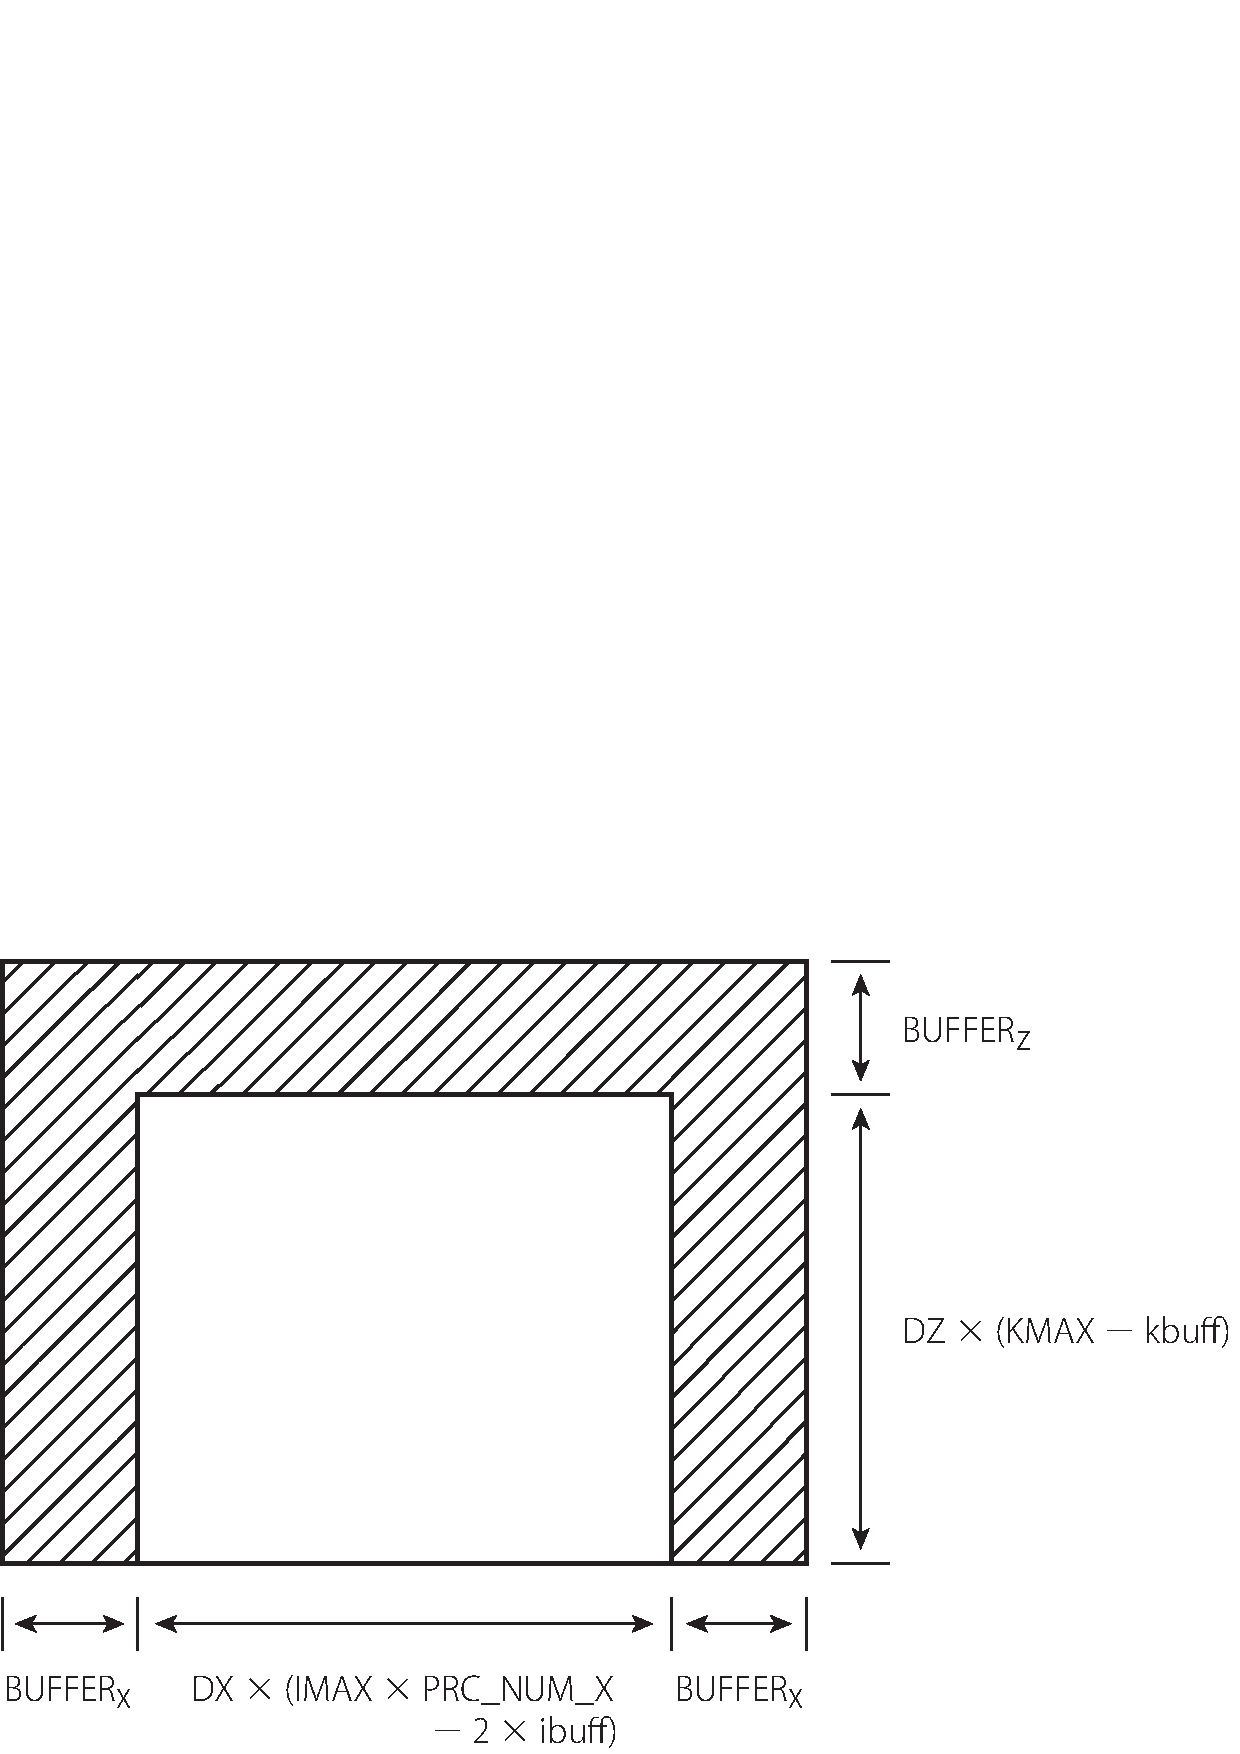
\includegraphics[width=0.8\hsize]{./figure/buffer_xz.pdf}\\
  \caption{全計算領域内での緩和領域の配置:斜線部分が緩和領域を意味する。
  図はXZ断面を示しているが、YZ断面についても同様である。}
  \label{fig:buff_xz}
\end{center}
\end{figure}

一般に、緩和領域の幅の設定や格子の置き方には明確な指標はない。
これらの設定は解く問題に依存する。
\scalerm では、モデル上部における鉛直方向の緩和領域の格子点数は5点以上、
側面境界の緩和領域の格子点は20〜40点程度を推奨している。
実験によっては、さらに緩和領域の格子点を増やしたり、
適切なストレッチ係数を用いて緩和領域自体を広げたり、
緩和の時定数を調整したりする必要があるだろう。
緩和の時定数については、以下で説明する。
%\namelist{PARAM_ATMOS_BOUNDARY}の中の
%\nmitem{ATMOS_BOUNDARY_taux, ATMOS_BOUNDARY_tauy, ATMOS_BOUNDARY_tauz}によって秒単位で設定する。
%\nmitem{ATMOS_BOUNDARY_taux, ATMOS_BOUNDARY_tauy}によって秒単位で設定する。
%デフォルトの値は、\nmitem{TIME_DT}の10倍であり、これは、10タイムステップで$1/e$になることに相当する。
%タイムステップについては、第\ref{sec:timeintiv}節を参照のこと。

%-----------------------------------------------------------------------
%\subsubsection{緩和領域における格子間隔のストレッチ設定}
%-----------------------------------------------------------------------

緩和領域の格子間隔は、デフォルトでは
\namelist{PARAM_ATMOS_GRID_CARTESC}の中の\nmitem{DX, DY, DZ}で指定した通りである。
ただし、\nmitem{BUFFFACT}に1以上に設定することによって、ストレッチさせることもできる。
格子間隔を等間隔で指定した場合は、この\nmitem{BUFFFACT}の設定は全方向に対して適用される。
各方向で別々に設定したい場合は、\nmitem{BUFFFACT_X, BUFFFACT_Y, BUFFFACT_Z}を指定する。
\nmitem{FZ(:)}を与えることで鉛直レベルを指定した場合(第\ref{subsec:gridinterv}節参照)は、
上記のストレッチの設定は{\ZDIR}には適用されない。

緩和領域内の格子間隔 (\verb|BDX|) は次の通り決定される。
\begin{eqnarray}
 \verb|BDX(|n\verb|)| &=& \verb|DX| \times \verb|BUFFFACT|^n \nonumber
\end{eqnarray}
ここで、$n$は緩和領域内の格子点番号を表し、計算領域の内側から外側へ向う番号である。
緩和領域の格子間隔は、
\nmitem{BUFFFACT=1.0}とした場合は内部領域と同じであり、
\nmitem{BUFFFACT=1.2}とした場合は内部から外側の領域に向かって1.2倍の割合で広がっていく。
\nmitem{BUFFFACT}の値は任意に設定できるが、計算不安定を避けるために 1.0から1.2 までの値が推奨される。

最後に、緩和領域の大きさ$\verb|BUFFER|_{\verb|X|}$は、
\[
  \verb|BUFFER|_{\verb|X|} = \nmitemeq{DX} \times \frac{ \nmitemeq{BUFFFACT}^{\texttt{\detokenize{ibuff}}}-1}{ \nmitemeq{BUFFFACT}-1 }
\]
となる。
%
緩和領域の幅\nmitem{BUFFER_DX}を同じに設定した場合でも、
\nmitem{BUFFFACT}を大きくすると緩和領域の格子数は少なくなる。
\nmitem{BUFFER_NX}を与えた場合は、緩和領域の幅のみが変わる。

\subsubsection{緩和領域におけるナッジングの方法}

緩和領域におけるナッジングの設定は、\namelist{PARAM_ATMOS_BOUNDARY}内のパラメータで行う。
境界データの種類は、\namelist{PARAM_ATMOS_BOUNDARY}内の\nmitem{ATMOS_BOUNDARY_TYPE}によって設定する(表\ref{tab:nml_atmos_boundary_type})。

\begin{table}[h]
\begin{center}
\caption{境界値データの種類の選択}
\label{tab:nml_atmos_boundary_type}
\begin{tabularx}{150mm}{lXX} \hline
  \rowcolor[gray]{0.9} 値 & 種類の説明 \\ \hline
  \verb|NONE|    & ナッジングしない \\
  \verb|CONST|   & 指定された定数値にナッジングする \\
  \verb|INIT|    & 初期値にナッジングする \\
  \verb|OFFLINE| & ファイルから読み込んだ値にナッジングする(時間変化なし) \\
  \verb|REAL|    & 親モデルまたは親領域の値にナッジングする(時間変化あり) \\
  \hline
\end{tabularx}
\end{center}
\end{table}


以下は、\namelist{PARAM_ATMOS_BOUNDARY}内のパラメータである.
\editboxtwo{
  \verb|&PARAM_ATMOS_BOUNDARY | & \\
  \verb| ATMOS_BOUNDARY_TYPE = 'NONE',         | & ; 境界値データの種類。表\ref{tab:nml_atmos_boundary_type}を参照。 \\
  \verb| ATMOS_BOUNDARY_IN_BASENAME = '',      | & ; 境界値データのファイル名 (\verb|OFFLINE| または\verb|REAL| type の場合)\\
  \verb| ATMOS_BOUNDARY_IN_CHECK_COORDINATES | \textbackslash \\
  ~~\verb|                   = .true.,| & ; 境界データファイル内の座標変数を確認するかのフラグ \\
  \verb| ATMOS_BOUNDARY_START_DATE | \textbackslash \\
  ~~\verb|        = (/ -9999, 0, 0, 0, 0, 0 /),| & ; 境界値データの開始時刻(\verb|REAL| type の場合のみ) \\
  \verb| ATMOS_BOUNDARY_UPDATE_DT = 0.0D0,     | & ; 境界値データの時間間隔(\verb|REAL| type の場合のみ) \\
  \verb| ATMOS_BOUNDARY_INTERP_TYPE | \textbackslash \\
  ~~\verb|                  = 'lerp_initpoint',| & ; 時間方向の補間の種類 \\
                                                 &  ~\verb|same_parent|: 最新の時間ステップでの値を使用 (補間なし), \\
                                                 &  ~\verb|nearest_neighbor|: 最も近い時間ステップでの値を使用, \\
                                                 &  ~\verb|lerp_initpoint|: 2つの時間ステップでの値を用いて瞬間値として線形補間する,  \\
                                                 &  ~\verb|lerp_midpoint|: \verb|lerp_initpoint|と同様であるが、境界データの時間ステップ間の時間平均値を使用 \\
  \verb| ATMOS_BOUNDARY_OUT_BASENAME = '',     | & ; 初期の境界値データを出力するファイル名 \\
  \verb| ATMOS_BOUNDARY_OUT_TITLE | \textbackslash \\
  ~~\verb|     = 'SCALE-RM BOUNDARY CONDITION',| & ; 出力ファイルに対するタイトル \\
  \verb| ATMOS_BOUNDARY_OUT_DTYPE = 'DEFAULT', | & ; 出力のデータ型(\verb|REAL4| or \verb|REAL8|) \\
  \verb| ATMOS_BOUNDARY_USE_DENS = .false.,    | & ; 密度に対するナッジングのスイッチ \\
  \verb| ATMOS_BOUNDARY_USE_VELZ = .false.,    | & ; wに対するナッジングのスイッチ. \\
  \verb| ATMOS_BOUNDARY_USE_VELX = .false.,    | & ; uに対するナッジングのスイッチ. \\
  \verb| ATMOS_BOUNDARY_USE_VELY = .false.,    | & ; vに対するナッジングのスイッチ. \\
  \verb| ATMOS_BOUNDARY_USE_POTT = .false.,    | & ; $\theta$に対するナッジングのスイッチ. \\
  \verb| ATMOS_BOUNDARY_USE_QV = .false.,      | & ; 水蒸気に対するナッジングのスイッチ. \\
  \verb| ATMOS_BOUNDARY_USE_QHYD = .false.,    | & ; 水物質に対するナッジングのスイッチ. \\
  \verb| ATMOS_BOUNDARY_VALUE_VELZ =   0.0D0,  | & ; wの値 (\verb|CONST| type の場合のみ) \\
  \verb| ATMOS_BOUNDARY_VALUE_VELX =   0.0D0,  | & ; uの値 (\verb|CONST| type の場合のみ) \\
  \verb| ATMOS_BOUNDARY_VALUE_VELY =   0.0D0,  | & ; vの値 (\verb|CONST| type の場合のみ) \\
  \verb| ATMOS_BOUNDARY_VALUE_POTT = 300.0D0,  | & ; $\theta$の値 (\verb|CONST| type の場合のみ) \\
  \verb| ATMOS_BOUNDARY_VALUE_QTRC =   0.0D0,  | & ; 水蒸気の値 (\verb|CONST| type の場合のみ) \\
  \verb| ATMOS_BOUNDARY_ALPHAFACT_DENS = 1.0D0,| & ; 密度に対する$1/\tau$の係数. \\
  \verb| ATMOS_BOUNDARY_ALPHAFACT_VELZ = 1.0D0,| & ; wに対する係数. \\
  \verb| ATMOS_BOUNDARY_ALPHAFACT_VELX = 1.0D0,| & ; uに対する係数. \\
  \verb| ATMOS_BOUNDARY_ALPHAFACT_VELZ = 1.0D0,| & ; vに対する係数. \\
  \verb| ATMOS_BOUNDARY_ALPHAFACT_POTT = 1.0D0,| & ; $\theta$に対する係数. \\
  \verb| ATMOS_BOUNDARY_ALPHAFACT_QTRC = 1.0D0,| & ; 水蒸気に対する係数. \\
  \verb| ATMOS_BOUNDARY_SMOOTHER_FACT = 0.2D0, | & ; 点ごとの差に対する水平方向の平滑化の係数. \\
  \verb| ATMOS_BOUNDARY_FRACZ = 1.0D0,         | & ; z方向の緩和領域に対するナッジング領域の割合. \\
  \verb| ATMOS_BOUNDARY_FRACX = 1.0D0,         | & ; x方向の割合. \\
  \verb| ATMOS_BOUNDARY_FRACY = 1.0D0,         | & ; y方向の割合. \\
  \verb| ATMOS_BOUNDARY_TAUZ = DT * 10.0D0,    | & ; 上端境界でのナッジングの時定数 (秒). \\
  \verb| ATMOS_BOUNDARY_TAUX = DT * 10.0D0,    | & ; 東西境界でのナッジングの時定数 (秒). \\
  \verb| ATMOS_BOUNDARY_TAUY = DT * 10.0D0,    | & ; 南北境界でのナッジングの時定数 (秒). \\
  \verb| ATMOS_BOUNDARY_LINEAR_V = .false.,    | & ; z方向に関するナッジングの時定数分布の種類. \verb|.true.|であれば線形分布、そうでなければサイン型の分布.\\
  \verb| ATMOS_BOUNDARY_LINEAR_H = .false.,    | & ; x, y 方向に関するナッジングの時定数分布の種類. \verb|.true.|であれば線形分布、そうでなければ指数関数分布. \\
  \verb| ATMOS_BOUNDARY_EXP_H = 2.0D0,         | & ; 指数関数分布の場合における指数の係数. \\
}

ナッジングによる時間変化率は、
\begin{eqnarray}
  \left.\frac{\partial \phi_{k,i,j}}{\partial t}\right|_\mathrm{nudging}
  & = & - \alpha \Delta\phi_{k,i,j} \\ \nonumber
  && + \alpha_s \left( \frac{\Delta\phi_{k,i-1,j} + \Delta\phi_{k,i+1,j} + \Delta\phi_{k,i,j-1} + \Delta\phi_{k,i,j+1}}{8} - \frac{\Delta\phi_{k,i,j}}{2} \right),
\label{eq:nudging}
\end{eqnarray}
と書かれる。
ここで、$\Delta\phi$ は境界値データとの差であり、
$\alpha_s = \alpha \times \nmitemeq{ATMOS_BOUNDARY_SMOOTHER_FACT}$である。
$\alpha$は3方向に対する係数$\alpha_x, \alpha_y,\alpha_z$の最大値である。
これらの係数は、以下のような長さスケール$e$に依存する。
\begin{equation}
  e = \max\left( 1 - \frac{d}{\texttt{BUFFER} \times \nmitemeq{ATMOS_BOUNDARY_FRAC}}, 0 \right),
\end{equation}
ここで、$d$は境界からの距離である。
もし\nmitem{ATMOS_BOUNDARY_LINEAR_V}が\verb|.true.|であれば、
\begin{equation}
  \alpha_z = e_z / \tau_z,
\end{equation}
\verb|.false.|であれば、
\begin{equation}
  \alpha_z =  \sin^2(\pi e_z/2) / \tau_z,
\end{equation}
である。
ここで、 $\tau_z$は\nmitem{ATMOS_BOUNDARY_TAUZ}である。
水平方向については、\nmitem{ATMOS_BOUNDARY_LINEAR_H}が\verb|.true.|であれば、
\begin{equation}
  \alpha_x = e_x / \tau_x,
\end{equation}
\verb|.false.|であれば、
\begin{equation}
  \alpha_x = e_x \exp\{ - (1-e_x) \times \nmitemeq{ATMOS_BOUNDARY_EXP_H} \} / \tau_x.
\end{equation}
である。
$\alpha_y$は$\alpha_x$と同様の方法によって導かれる。

$\tau$は境界($d=0$)での緩和時間であり、計算された値と境界値の差はこの時間スケールで$1/e$倍となる。
他方、式\ref{eq:nudging}の右辺2項目によって、$\Delta \phi$の two-grid スケールの成分は$\tau/\nmitemeq{ATMOS_BOUNDARY_SMOOTHER_FACT}$の時間で$1/e$倍となる。
$\tau$のデフォルトの値は、\nmitem{TIME_DT}の10倍である。
\nmitem{TIME_DT}については第\ref{sec:timeintiv}節を参照されたい。


\namelist{PARAM_ATMOS_BOUNDARY}内の\nmitem{ATMOS_BOUNDARY_TYPE}が\verb|REAL|であれば、
水平速度・温位・水蒸気に対する側面境界でのナッジングが強制的に適用される。
この場合は、\nmitem{ATMOS_BOUNDARY_USE_VELX}, \nmitem{ATMOS_BOUNDARY_USE_VELY},
\nmitem{ATMOS_BOUNDARY_USE_POTT}, \nmitem{ATMOS_BOUNDARY_USE_QV} といったスイッチは、上端境界に対してのみ使われる。
オンライン・ネスティング(第\ref{subsec:nest_online}節を参照)の子領域で計算が行われるときには、
境界の種類として\verb|REAL|を用いて上記と同様の設定が適用される。

上端境界の周辺における同様な減衰のさせ方として、レイリー摩擦が存在する(第 \ref{subsec:raydamp}節を参照)。
